\documentclass[tikz]{standalone}

\usepackage{listings}
\usepackage{luatex85}

\usetikzlibrary{shapes.multipart}
\usetikzlibrary{matrix}
\usetikzlibrary{positioning}
\usetikzlibrary{fit}
\usetikzlibrary{chains}
\usetikzlibrary{graphs}

\tikzset{
%  abc
 deprecated/.style={draw, gray!90!black}
}

\tikzset{
 class/.style={draw, rectangle split, rounded corners, 
  rectangle split parts=3, 
  % Currently one must explicitly specify the colours for each 
  % cell as is shown below, but it ought to be possible to use 
  %
  %   rectangle split use custom fill=true,
  %   every PART nodepart/.style={red},
  %
  % It should further be possible to specify the parts colour 
  % in the \nodepart macro as in
  %
  %   \node[rectangle split] {First \nodepart[fill=red]{second} Second};
  %
  % As I have not managed to get either method to work I use 
  % the following key, which sets 
  %
  %   rectangle split use custom fill
  %
  rectangle split part fill ={{gray!50!white}, gray!15!white, gray!15!white},
  rectangle split part align={center, left, left},
  % One may either explicitly ignore empty parts as follows or
  % manipulate their dimensions using the keys :
  %
  % rectangle split empty part height = 0.1em,
  % rectangle split empty part depth  = 0.1em,
  rectangle split ignore empty parts=true,
  }
}

\begin{document}

% PEP 420 - Name Spaced Packages
% PEP 302 - sys.Meta_Path implementation

% The \href{https://docs.python.org/3/reference/import.html}{import system} roughly follows the following scheme.
% section 5.4.2 Submodules explains binding of submodules by a parent during imports.

% During an import the parts of module name are traversed in sequence \nixpath{first.second}


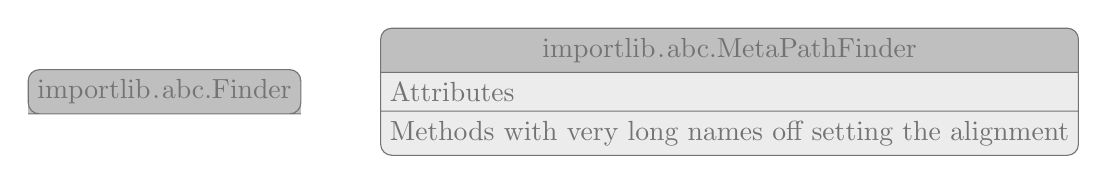
\begin{tikzpicture}[
 start chain, 
 %deprecated/.style = {top color = grey}
]
\node[on chain, class, deprecated] {\lstinline|importlib.abc.Finder|};
\node[on chain, class, deprecated] {\lstinline|importlib.abc.MetaPathFinder| \nodepart{second} Attributes \nodepart[fill= green]{third} Methods with very long names off setting the alignment};
\end{tikzpicture}

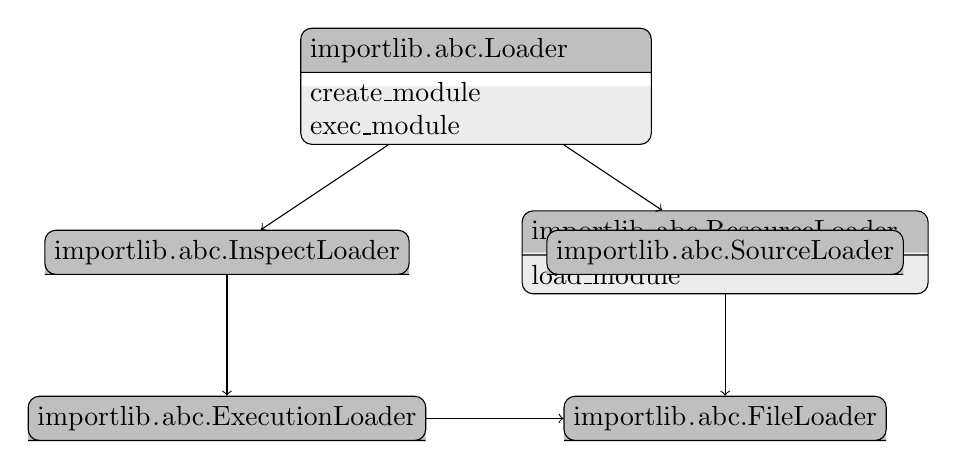
\begin{tikzpicture}[
 start chain, 
 %deprecated/.style = {top color = grey}
]
\node[text width = 12em, class] (ploader) at (0em,24em) {\lstinline|importlib.abc.Loader| \nodepart{third} \lstinline|create_module| \\ \lstinline|exec_module|}; % Python >= 3.4
% \node[text width = 12em, class] (ploader) at (0em,24em) {\lstinline|importlib.abc.Loader| \nodepart{third} \lstinline|load_module| \\ \lstinline|module_repr|};   % Python <= 3.4
\node[text width = 14em, class] (rloader) at ( 9em,18em) {\lstinline|importlib.abc.ResourceLoader| \nodepart{third} \lstinline|load_module|};
\node[class] (iloader) at (-9em,18em) {\lstinline|importlib.abc.InspectLoader|};
\node[class] (eloader) at (-9em,12em) {\lstinline|importlib.abc.ExecutionLoader|};
\node[class] (floader) at ( 9em,12em) {\lstinline|importlib.abc.FileLoader|};
\node[class] (sloader) at ( 9em,18em) {\lstinline|importlib.abc.SourceLoader|};
\graph {(ploader) -> {(rloader), {(iloader) -> (eloader)}} -> (floader); 
%         {(rloader), (eloader)} -> (sloader); 
        
        };
% Note that one may use the _register function to tak on a MetaPath finder
\end{tikzpicture}

% \begin{tikzpicture}[
%  object/.style   = {draw, rounded corners},
%  alternatives/.style = {object, rectangle split, rectangle split parts=#1, anchor=center},
% ]
% \node[alternatives=3, label=below:Entry Point, label=above:Fully Qualified Module Name (FQMN)] (ep) at (-10em,10em) {\lstinline|import| \nodepart{two} \lstinline|__import__()| \nodepart{three} \lstinline|importlib.import_module()|};
% \node[object, label=below:Module Cache]    (sm) at ( 10em, 10em) {\lstinline|sys.modules|};
% % \node[label=below:]                     at ( 10em,-10em) {\lstinline|sys.path|};
% \node[alternatives=3, label=above:\lstinline|sys.MetaPath|, label=below:Importers] (mp) at ( 10em,0em) {Builtins \nodepart{two} Frozen \nodepart{three} importlib.machinery.PathFinder (URI/URLs)};
% \node[alternatives=3, label={[above, text width = 8em, align=center] \\ }, label=below:Finders] (finders) at ( 10em,-10em) {\lstinline|find_spec()| \nodepart{two} \lstinline|find_module()| \nodepart{three}};
% \node[alternatives=2, label=above:Module,label=below:Loaders] (loaders) at (-10em,-10em) {\lstinline|load_module| \nodepart{two} \lstinline|exec_module|};
% \node[object,         label=above:Importers, rotate fit = 0, fit = (finders) (loaders), inner sep = 2em] {};
% \draw[->] (ep) to[out=0, in=180]   (sm);
% \draw[->] (sm) to[out=0, in=  0] (mp);
% \draw[->]  (finders) --node[above] {Mod. Spec.} node[below] {Loader ($\le$ 3.4)} (loaders);
% \end{tikzpicture}

% \begin{tikzpicture}
% \node {import}; 
% \node {search \lstinline|sys.modules|};
% \node {search \lstinline|sys.meta_path|};
% \end{tikzpicture}

% \begin{tikzpicture}[inner sep = 0, outer sep=0]
% %  subclass/.style = {rectangle split, rectangle split parts=#1, draw, anchor=center, rounded corners}
% % ]
% % \node {\lstinline|fing_spec|};
% % \node[subclass=3, label=above:, label=below:] {\lstinline|first.second.third| \nodepart{two} \lstinline|first| \lstinline|second.third| \nodepart{three} \lstinline|importlib.import_module|};
% \coordinate                (lvl1) {};
% \coordinate[below=of lvl1] (lvl2) {};
% \coordinate[below=of lvl2] (lvl3) {};
% \coordinate[below=of lvl3] (lvl4) {};
% \node[right = of lvl1] (fqmn) {\lstinline|first.second.third|};
% \node[right = of lvl2] (f)    {\lstinline|first|};              % \node[node distance =0.5em,right = of  f] (st) {\lstinline|second.third|};
% \node[right = of lvl3] (fs)   {\lstinline|first.second|};       % \node[node distance =0.5em,right = of fs]  (t) {\lstinline|third|};
% \node[right = of lvl4] (fst)  {\lstinline|first.second.third|};
% \end{tikzpicture}

% The idea here is to return None or a spec. 
% If None is returned the system proceeds to investigate other sources (MetaPath and Path based \empg{importers}) 
% Otherwise a spec must be created. 
% This follows one of two routes, create a loader and generate a spec from this or create a spec directly from a file.
% The former is more flexable as it allows one to select between various loader classes.
% \begin{tikzpicture}
% \node (loader) {\lstinline|loader|};
% \node (lspec)  {\lstinline|spec_from_loader|};
% \node (fspec)  {\lstinline|spec_from_file|};
% \node[fit = (fspec) (lspec) ] {};
% \end{tikzpicture}

\end{document}